% !TEX encoding = UTF-8
% !TEX TS-program = pdflatex
% !TEX root = ../tesi.tex

%**************************************************************
\chapter{Descrizione architettura software}
\label{cap:descrizione-architettura}
%**************************************************************

\intro{In questo capitolo verrà descritta l'architettura software del gestionale SAP e dei moduli aggiunti dall'azienda}\\
%**************************************************************
\begin{figure}[!h] 
	\centering 
	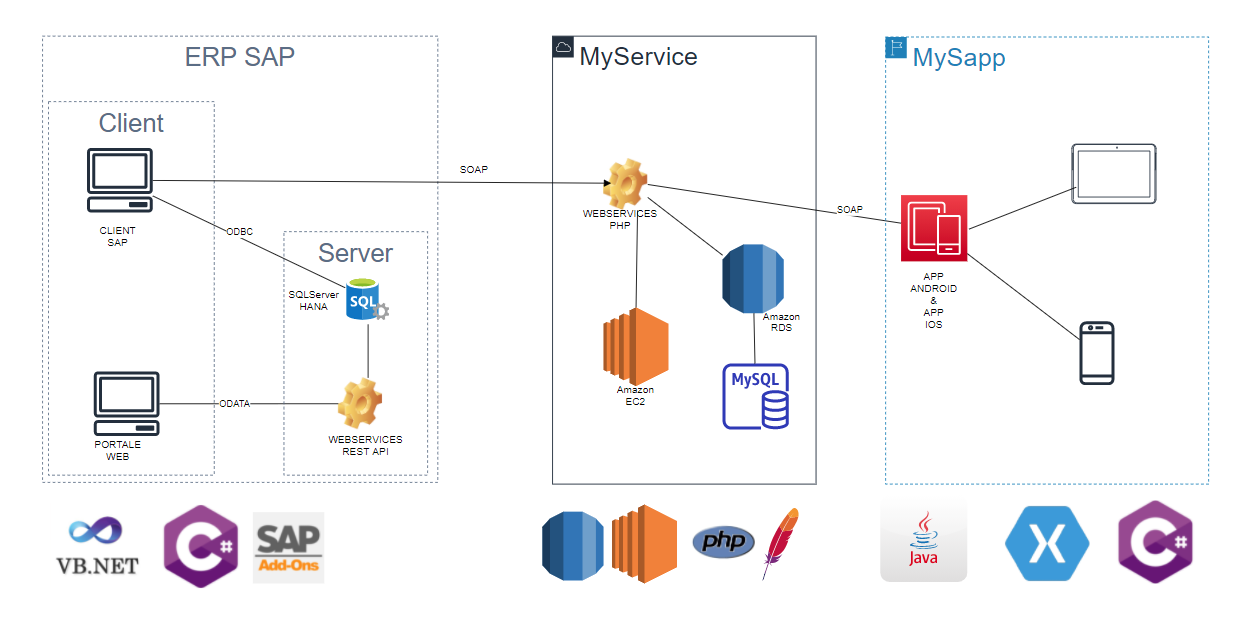
\includegraphics[scale = 0.4]{immagini/architettura-globale.png} 
	\caption{Schema di rappresentazione modulo gestionale ERP SAP, e moduli aggiunti dall'azienda intorno al gestionale}
\end{figure}\\
Da quest'immagine possiamo notare i tre moduli principali:
\begin{itemize}
	\item \textbf{ERP SAP:} il modulo del gestionale;
	\item \textbf{MyService:} il modulo dei webservices AWS;
	\item \textbf{MySapp:} il modulo delle applicazioni Android e iOS.\\
\end{itemize}
Sulle due parti evidenziate dal cerchio rosso si è basato il mio lavoro in questo stage.
Nel client SAP verrà applicato l'applicazione add-on, mentre nei webservices php sono state effettuate delle modifiche ad alcune funzioni.
\section{Descrizione modulo ERP SAP}
\begin{figure}[!h] 
	\centering 
	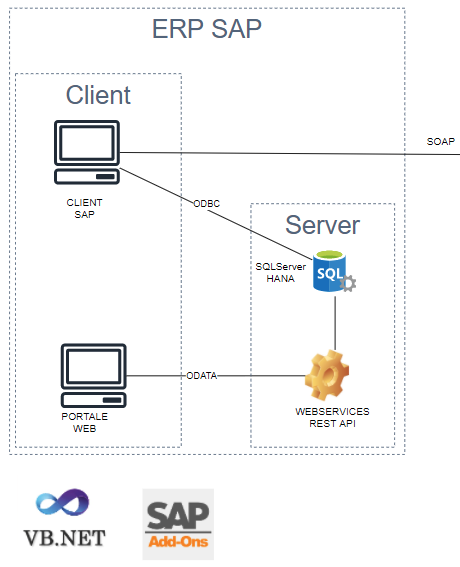
\includegraphics[scale = 1.2]{immagini/modulo-sap.png} 
	\caption{Schema di rappresentazione modulo gestionale ERP SAP}
\end{figure}

\subsection{ERP SAP}
\vspace{1em}
ERP SAP rappresenta il modulo del gestionale, in particolare nel nostro caso abbiamo come gestionale il SAP Business One.\\
ERP è l'acronimo di Enterprise Resource Planning.\\SAP è l'acronimo di Systems, Applications, Products.\\\\
SAP è un'azienda leader nel settore di ERP, e i suoi prodotti sono dei gestionali, ovvero dei software ERP.\\\\
Un software ERP è un tipo di software che le organizzazioni utilizzano per gestire le attività commerciali quotidiane, come ad esempio contabilità, project management, gestione del rischio e operazioni e gestione della catena di distribuzione.\\\\
Come possiamo vedere in Figura 2.2, il SAP è suddiviso in client e server.\\
Il server può essere basato su :
\begin{itemize}
	\item \textbf{SQLServer:} solo su Windows;
	\item \textbf{HANA:} solo su Linux.
\end{itemize}
Il client SAP attualmente è disponibile solo su Windows.\\Sul client SAP possono essere applicati degli add-on, per modificare i comportamenti della GUI del client in base a com'è programmato l'add-on.\\\\
I due gestionali più famosi di SAP sono:
\begin{itemize}
	\item SAP R/3;
	\item SAP Business One.
\end{itemize}
Questo progetto di stage è stato incentrato intorno al SAP Business One, dunque ora entreremo più nel dettaglio, su quest'ultimo.
\newpage
\subsection{SAP Business One}
SAP Business One, abbreviato a SAB B1, è un sofware ERP basato sulle piccole/medie imprese.
\\\\Questo gestionale è attualmente alla versione 10, rilasciata a marzo 2020, e rispetto al SAP R/3 consente molte più personalizzazione per essere adatto alle esigenze più disparate.
\\\\Come detto in precedenza è un tipico software con modello Client-server.
\begin{itemize}
	\item Il client è principalmente il Client SAP, o B1 Client, ma può essere anche un portale web oppure un'applicazione mobile;
	\item Il server viene eseguito su un database Microsoft SQL Server (Windows) oppure un database SAP HANA (Linux).\\
\end{itemize}
Infine, come detto in precedenza, SAB B1 consente di effettuare molte personalizzazioni (ovvero gli add-on) utilizzando \textbf{SAP Business One SDK}, ovvero un insieme di strumenti e librerie disponibili per lo sviluppo di add-ons su Microsoft Visual Studio, con C\# o VB.NET.\\\\
\begin{figure}[!h] 
	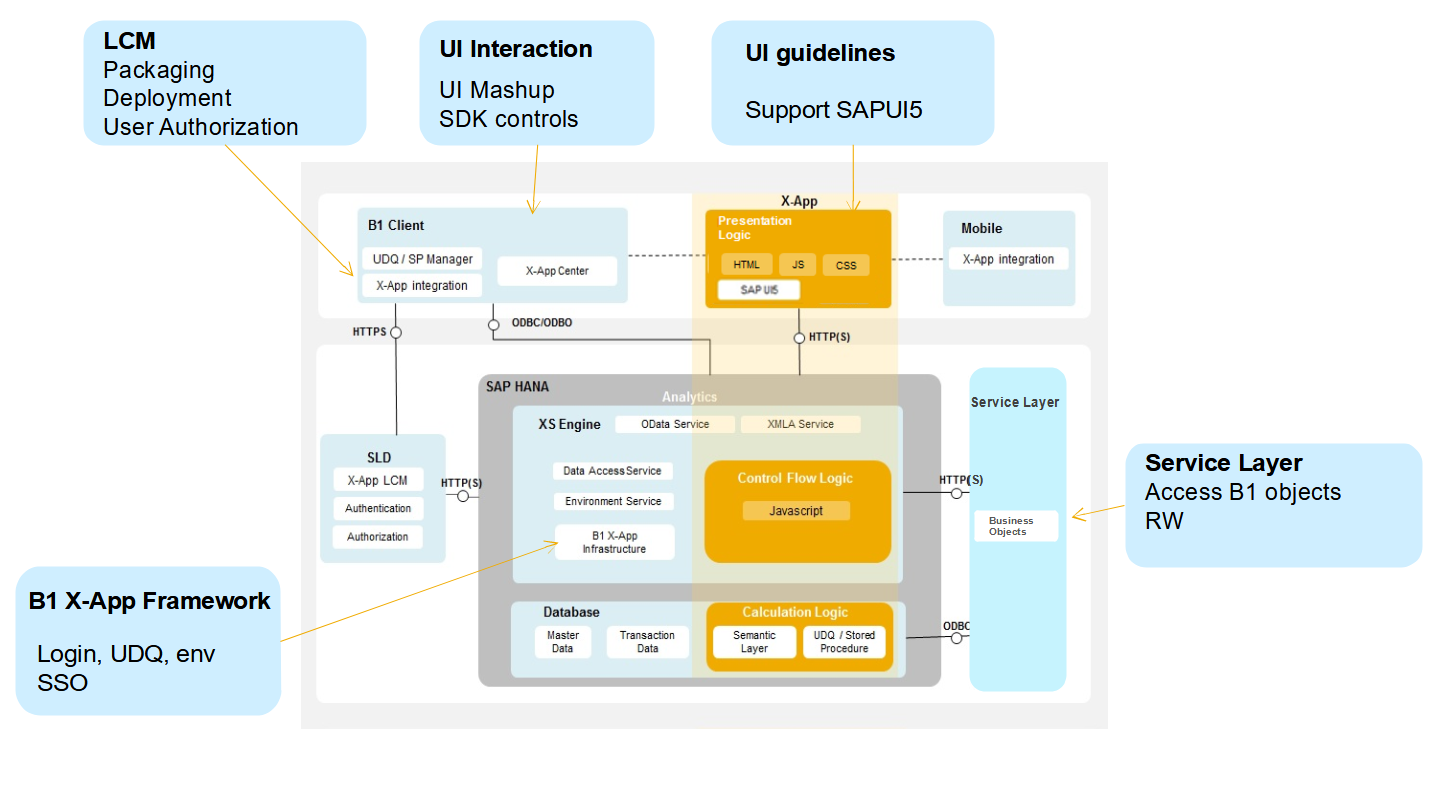
\includegraphics[scale = 0.4, left]{immagini/erp-sap-inside.png} 
	\caption{Schema ufficiale sul SAP Business One}
\end{figure}
\newpage
Qui possiamo vedere uno schema sul SAP Business One, ufficiale dalla documentazione SAP.\\
Possiamo vedere i vari client con cui accedere al SAP:
\begin{itemize}
	\item \textbf{B1 Client:} ovvero il client SAP desktop;
	\item \textbf{X-APP:} ovvero un portale web sviluppato da SAP;
	\item \textbf{X-APP per mobile:} l'integrazione X-APP, per i dispositivi mobile;
	\item \textbf{Service Layer:} i webservices REST API, che possono essere utilizzati a loro volta da altre applicazioni (ad esempio, sito web o applicazioni mobile), per accedere al SAP.
\end{itemize}
Tutti questi client accedono al SAP attraverso vie diverse.
\begin{itemize}
	\item Il client SAP, B1 Client, accede al database attraverso ODBC (oppure ODBO), e accede a SLD, ovvero la componente di autenticazione, via HTTP(S);
	\item I webservices accedono al server SAP attraverso HTTP(S), e ricevono risposta dal database attraverso ODBC;
	\item X-APP, sia versione web che mobile, accede al server SAP, e quindi successivamente al database, attraverso HTTP(S).
\end{itemize}
In questa figura, si può XS Engine, ovvero il server SAP (la logica SAP) e il database, contenuti dentro il DBMS SAP HANA, ma lo stesso vale se il DBMS è Microsoft SQL Server.\\
Ora proseguiamo analizzando le componenti principali del SAP, ovvero:
\begin{itemize}
	\item il client SAP;
	\item il server SAP;
	\item il Service Layer di SAP, ovvero i webservices REST API.
\end{itemize}
\newpage
\subsection{Client SAP}
\begin{flushleft}
	\item Il client SAP utilizza la connessione ODBC per comunicare con il server SAP.\\ODCB, ovvero Open DataBase Connectivity, è uno standard utilizzato per la connessione tra client e DBMS. 
	\item Mentre utilizza il protocollo SOAP per comunicare con il webserver AWS del modulo MyService.
\end{flushleft}
\begin{figure}[!h] 
	\centering 
	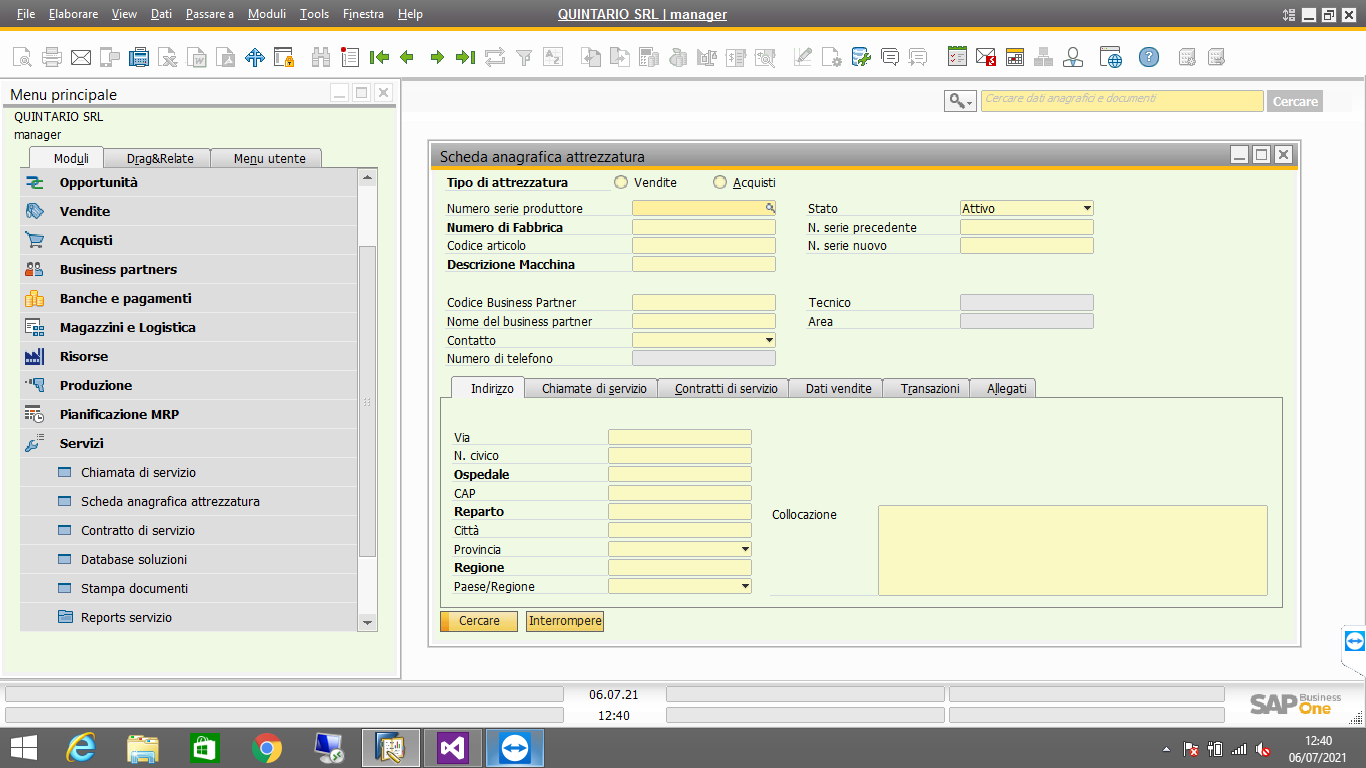
\includegraphics[scale = 0.4]{immagini/client-sap.png} 
	\caption {Client SAP, aperto sulla scheda "Scheda anagrafica attrezzatura"}
\end{figure}
\begin{flushleft}
	\item Qui possiamo vedere come appare il Client SAP.\\In questo caso è stata aperta la Scheda anagrafica attrezzatura, del modulo dei Servizi.\\Da notare che questi "moduli" del SAP, differiscono dai moduli coinvolti con il modulo del gestionale (MyService e MySapp), questi sono moduli interni del SAP.
	\item La scheda anagrafica attrezzatura è una scheda che rappresenta le attrezzature dell'azienda, ad esempio macchine a controllo numerico, lavatrici o condizionatori, e tutti i possibili macchinari dell'azienda.
	\item Ora vediamo un esempio di cambiamento della GUI di questo client con l'applicazione di un Add-On alla scheda anagrafica attrezzatura.
\end{flushleft}
\pagebreak
\begin{figure}[!h] 
	\centering 
	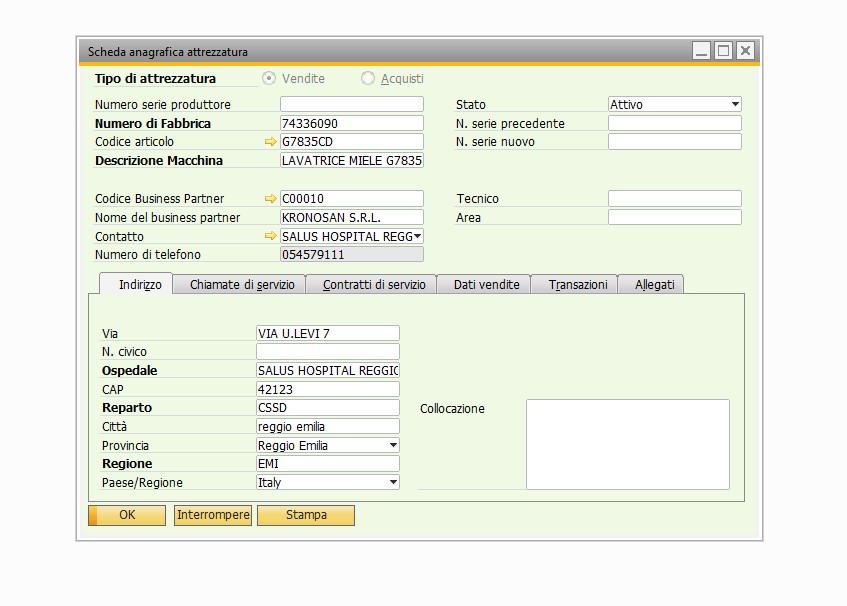
\includegraphics[scale = 0.6]{immagini/esempio-modifica-client-addon.jpg} 
	\caption {Client SAP, esempio di modifica GUI di un add-on applicato sulla scheda "Scheda anagrafica attrezzatura"}
\end{figure}
\begin{flushleft}
	\item Come possiamo vedere è apparso un nuovo pulsante, che stamperà i dati della scheda.\\Questo è un'esempio molto semplice, ma si possono cambiare altre cose, ad esempio aggiungere o rimuovere campi, o aggiungere funzioni ad eventi, ad esempio messaggi di testo che appaiono cliccando dei campi particolari.
\end{flushleft}
\newpage
\subsection{Portale Web}
Ora mostriamo il portale web, sviluppato dall'azienda, in concomitanza con un'altra azienda specializzata in siti web (mys).\\
L'admin del portale, oppure l'admin relativo all'azienda cliente, crea le credenziali per i vari utenti, che saranno i dipendenti delle aziende clienti di Sinapsi.\\
Dunque arrivati al sito web, bisogna inserire le credenziali nella sezione Login, che apparirà come prima pagina del sito.\\
\begin{figure}[!h] 
	\centering 
	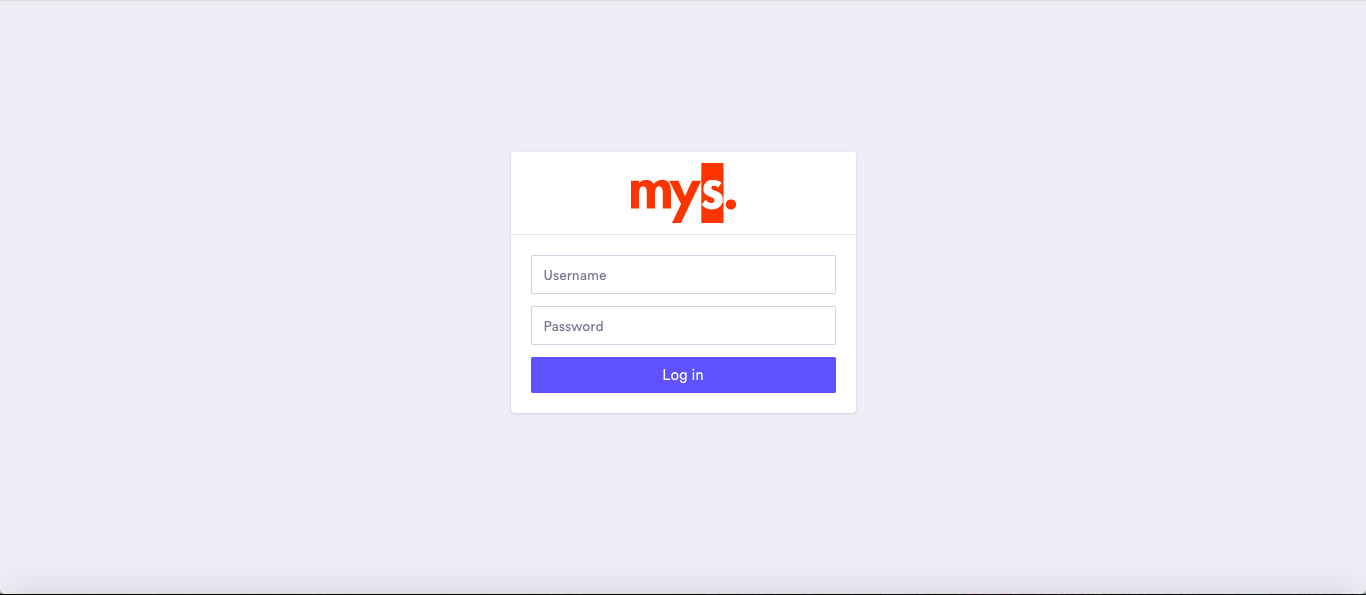
\includegraphics[scale = 0.6]{immagini/portale/login.png} 
	\caption {Portale Web, sezione di Login}
\end{figure}
Una volta effettuato il login, si viene reindirizzati al sito web, vero e proprio.\\
Da qui abbiamo principalmente 3 schermate principali:
\begin{itemize}
	\item Attrezzature;
	\item Calendario;
	\item Interventi.
\end{itemize}
Cominciamo con la schermata Calendario, qui sotto.
\begin{figure}[!h] 
	\centering 
	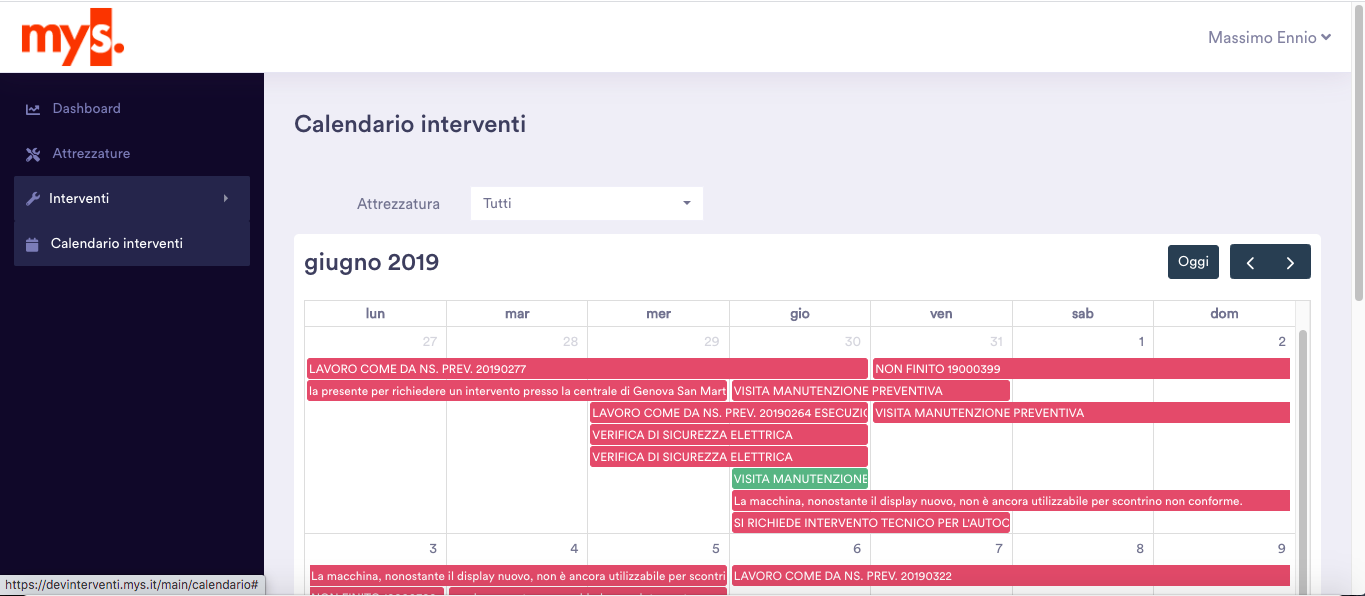
\includegraphics[scale = 0.6]{immagini/portale/calendario.png} 
	\caption {Portale Web, schermata Calendario}
\end{figure}
Evidenziate di rosso ci sono le chiamate di servizio, ad esempio manutenzioni, non completate, mentre evidenziate in verde quelle completate.\\
Ora continuiamo con la schermata Attrezzature.
\begin{figure}[!h] 
	\centering 
	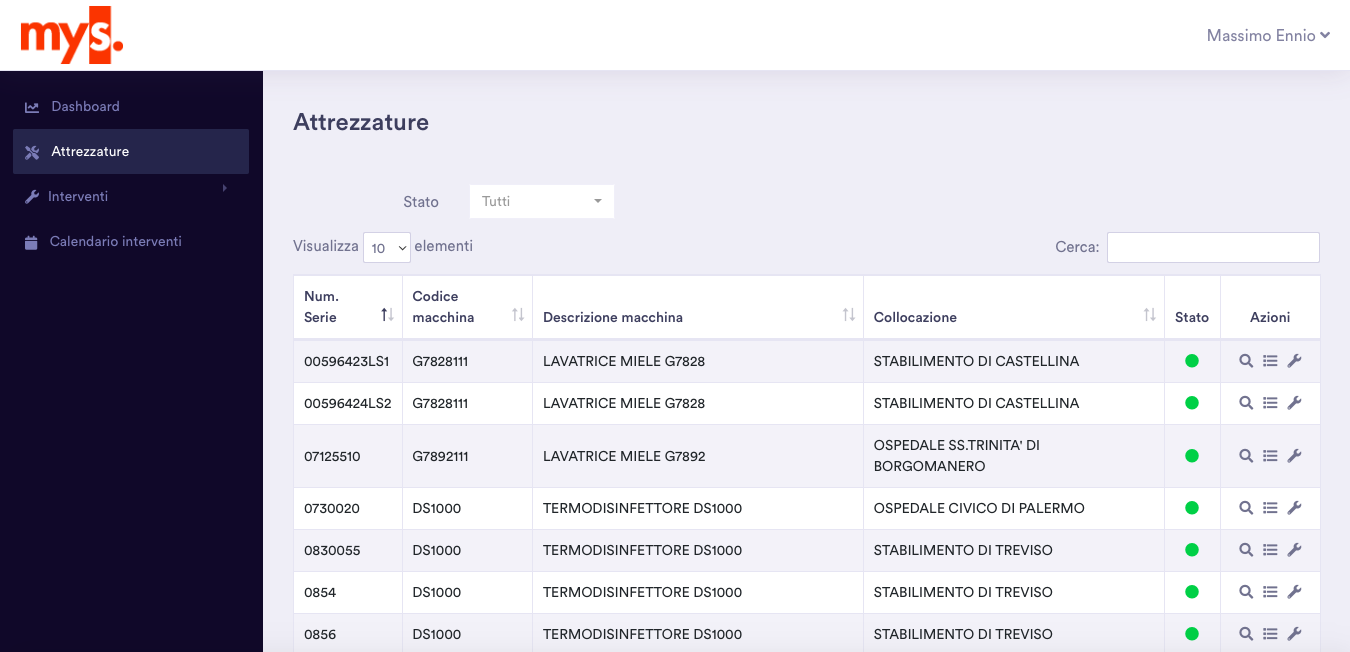
\includegraphics[scale = 0.6]{immagini/portale/attrezzature.png} 
	\caption {Portale Web, schermata Attrezzature}
\end{figure}
Qui possiamo vedere tutte le attrezzature, relative all'azienda cliente collegata, e quindi alle credenziali.\\
Per ogni attrezzature ci sono alcune azioni, tra cui ricerca ed elenco chiamate di servizio.\\Tra le varie azioni la più interessante è l'apertura di una nuova chiamata di servizio, ovvero richiedere un nuovo intervento, ad esempio una manutenzione o sostituzione di componenti.\\\\
Ora passiamo alla schermata degli interventi, di cui possiamo conoscerne tutte le caratteristiche principali, come numero di intervento, tipo di intervento, data inizio e fine.\\
E anche la causale e lo stato, per stato si intende se l'intervento è già stato effettuato.\\\\Infine, all'interno della schermata degli interventi, abbiamo la sezione "In attesa", per gli interventi in attessa di sincronizzazione.
\begin{figure}[!h] 
	\centering 
	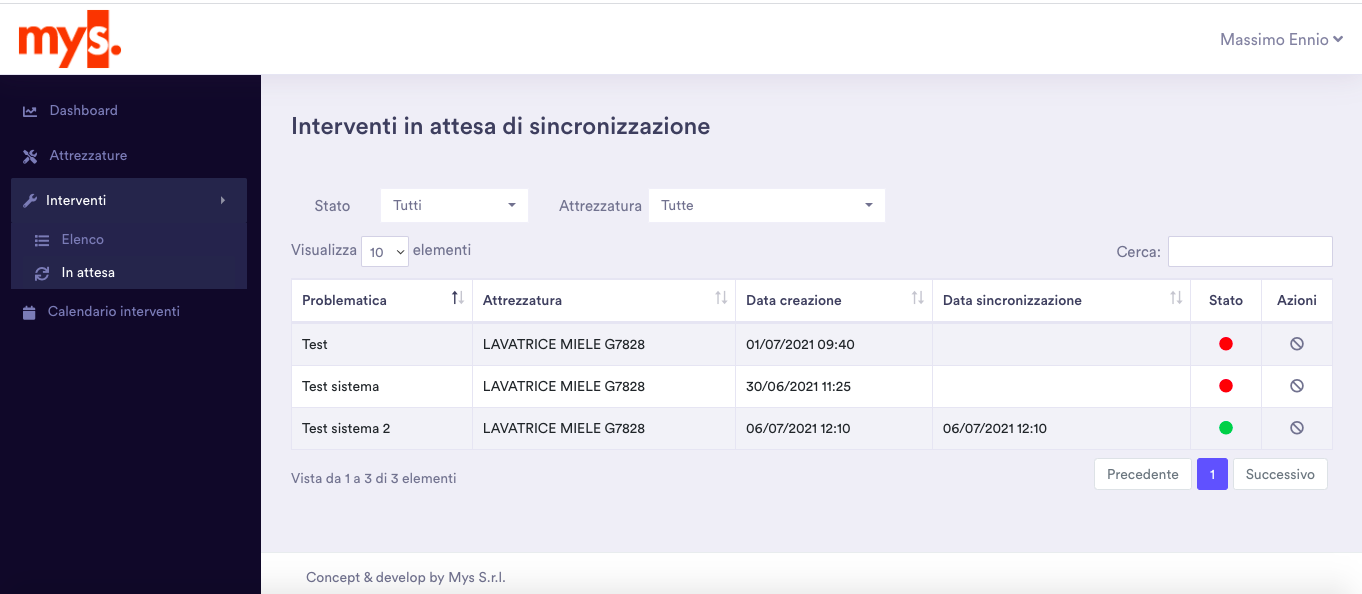
\includegraphics[scale = 0.6]{immagini/portale/interventi-in-attesa.png} 
	\caption {Portale Web, sezione di Login}
\end{figure}
\begin{figure}[!h] 
	\centering 
	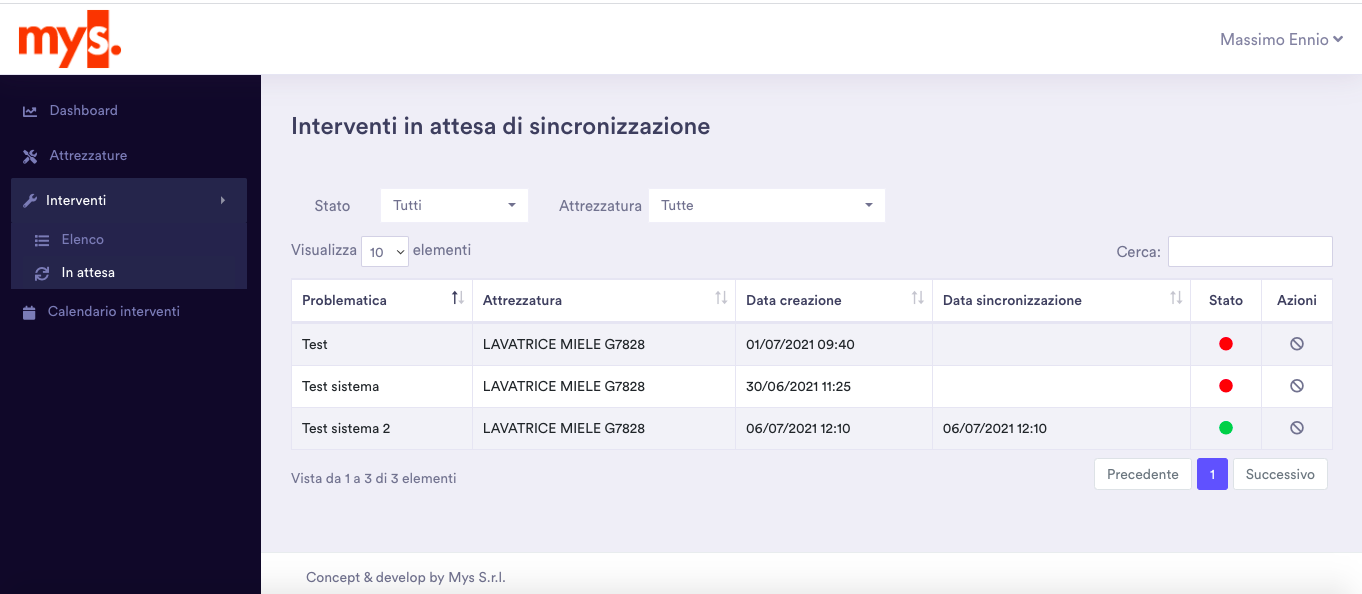
\includegraphics[scale = 0.6]{immagini/portale/interventi-in-attesa.png} 
	\caption {Portale Web, schermata Interventi, sezione In attesa}
\end{figure}

\pagebreak
\subsection{Webservices REST API}
\begin{flushleft}
	\item Recentemente, su SAP Business One è stato introdotto un service layer, composto da webservices REST API, che comunicano tramite protocollo ODATA (open data protocol).
	\item Questi webservices permettono di accedere direttamente agli oggetti SAP,\\senza passare per il client SAP.\\Gli oggetti SAP sono una struttura dati generata dalla logica del server SAP, \\che raggruppano e ordinano secondo certe logiche i dati presenti nel database.
	\item Per poter ottenere questi dati bisogna fare una richiesta http al webserver, il quale invierà un file json con gli oggetti SAP richiesti.
	\item L'utilizzo più comune di questi webservices è un portale web che usi le informazioni prese tramite queste richiete HTTP. 
\end{flushleft}
\begin{figure}[!h] 
	\centering 
	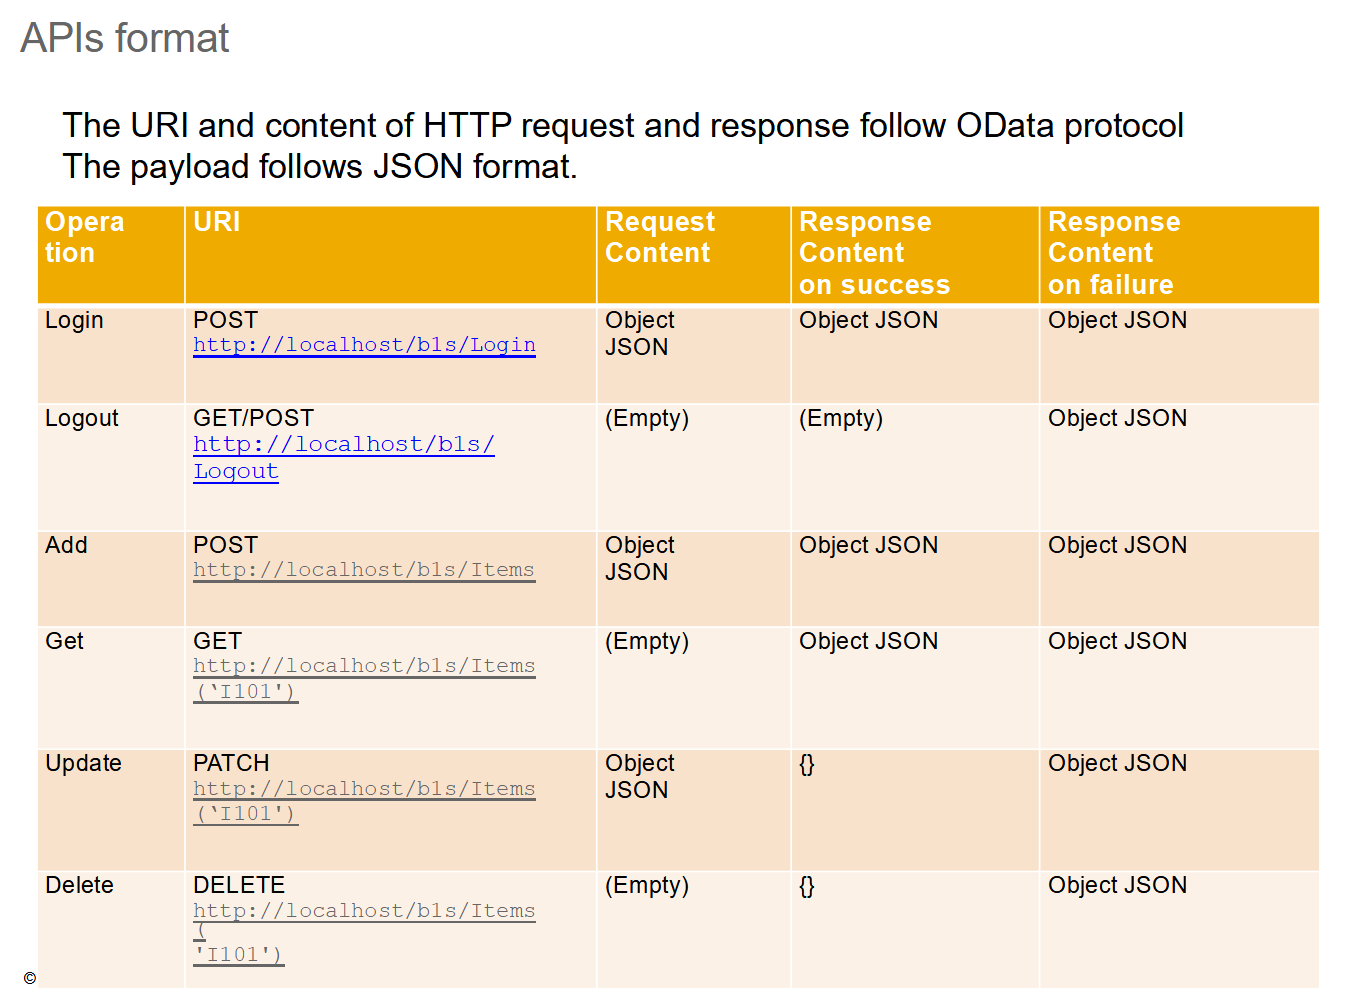
\includegraphics[scale = 0.4]{immagini/api_Format.png} 
	\caption {Formato delle richieste HTTP per il Service Layer SAP}
\end{figure}
\begin{flushleft}
	\item Come si può osservare da quest'immagine, sono presenti le richieste HTTP principali per interagire con i webservices REST API del Service Layer di SAP.
	\item A seguito di una richiesta HTTP viene elaborata la richiesta.\\Viene restituito un oggetto JSON in caso di fallimento, comunicando l'errore causante il fallimento.\\In caso di successo viene restituito un oggetto JSON, ove necessario, oppure un messaggio vuote che rappresenta il successo dell'operazione.
\end{flushleft}



